%Thedore Ian Martiny
%Summer 2016 Test 2 Review

\documentclass[addpoints]{exam}
\newcommand{\naturals}{\mathbb{N}}
\newcommand{\integers}{\mathbb{Z}}
\newcommand{\reals}{\mathbb{R}}
\renewcommand{\baselinestretch}{1.5}
%\setlength{\textwidth}{16cm}
\usepackage{amsfonts}
\usepackage{amsmath}
\usepackage{amsthm}
\usepackage{amssymb}
\usepackage{color}
\usepackage{colortbl}
\usepackage{fullpage}
\usepackage{graphicx}
\usepackage[utf8]{inputenc}
\usepackage{listings}
\usepackage{multicol}
\usepackage{setspace}
\usepackage{wasysym}
\usepackage{xcolor}
 
\definecolor{codegreen}{rgb}{0,0.6,0}
\definecolor{codegray}{rgb}{0.5,0.5,0.5}
\definecolor{codepurple}{rgb}{0.58,0,0.82}
\definecolor{backcolour}{rgb}{0.95,0.95,0.92}
\definecolor{Gray}{gray}{0.85}
 
\lstdefinestyle{mystyle}{
    backgroundcolor=\color{backcolour},   
    commentstyle=\color{codegreen},
    keywordstyle=\color{magenta},
    numberstyle=\tiny\color{codegray},
    stringstyle=\color{codepurple},
    basicstyle=\footnotesize,
    breakatwhitespace=false,         
    breaklines=true,                 
    captionpos=b,                    
    keepspaces=true,                 
    numbers=left,                    
    numbersep=5pt,                  
    showspaces=false,                
    showstringspaces=false,
    showtabs=false,                  
    tabsize=2
}
\newcolumntype{a}{>{\columncolor{Gray}}c} 
\lstset{style=mystyle}
\begin{document}
\singlespacing

\begin{center}
  {\large\textbf{CSCI 2824 - Discrete Structures}}

  {\large\textbf{Test 2 Review}}
\end{center}

\begin{questions}
  \question For the following determine if $A = B$
  \begin{parts}
    \part $C = \{1,2,3\}$, $D = \{2,3,4\}$, $A = \{2,3\}$, $B = C\cap D$.
    \vspace*{\fill}
    \begin{solution}
      $C \cap D = \{2,3\}$ so yes $A = B$.
    \end{solution}

    \part $A = \{1,2,3\}$, $B = \{n : n \in \integers^+ \text{ and } n^2 < 10\}$
    \vspace*{\fill}
    \begin{solution}
      Note that $1^2 = 1  <10$, $2^2 = 4 < 10$, $3^2 = 9 < 10$ so $B = \{1,2,3\}$ so yes $A = B$.
    \end{solution}

    \part $A = \{1,3,5\}$, $B = \{n : n \in \integers^+ \text{ and } n^2 - 1 < n\}$
    \vspace*{\fill}
    \begin{solution}
      Note that $1^2 -1 = 0 < 1$, but $3^2 - 3 = 6 > 3$ so $3\not\in B$ so $A\not= B$.
    \end{solution}

    \part $A = \{x : x \in \reals \text{ and } 0 \leq x \leq 2\}$, $B = \{1,2\}$.
    \vspace*{\fill}
    \begin{solution}
      No. $A$ is all \textbf{real} numbers between 0 and 2, where as $B$ is just the integers 1, and 2.
    \end{solution}
  \end{parts}

  \question For the following questions use represent the propositions using the given symbols, and determine whether the proposition is true or not.
  \begin{center}
    $p: 5 < 9$

    $q: 9 < 7$

    $r: 5 < 7$
  \end{center}

  \begin{parts}
    \part $5 < 9$ and $9 < 7$
    \vspace*{\fill}
    \begin{solution}
      $p\wedge q$ this is false, $9 > 7$.
    \end{solution}

    \part It is not the case that ($5<9$ and $9 < 7$)
    \vspace*{\fill}
    \begin{solution}
      $\neg(p\wedge q)$ this is true since $p\wedge q$ is false.
    \end{solution}
  \end{parts}

  \question For the following questions assume that $p$ and $r$ are false and that $q$ and $s$ are true. Determine the truth value of the given proposition.
  \begin{parts}
    \part $(p \to r) \wedge (q\to r)$
    \vspace*{\fill}
    \begin{solution}
      Since $p$ is false then $p\to r$ is true. However since $q$ is true and $r$ is false then $q\to r$ is false. This makes the proposition false.
    \end{solution}

    \part $p\to (q\to r)$
    \vspace*{\fill}
    \begin{solution}
      Since $p$ is false then this is vacuously true.
    \end{solution}

    \part $(s \to (p \wedge \neg r)) \wedge ((p \to (r \vee q)) \wedge s)$
    \vspace*{\fill}
    \begin{solution}
      The first clause on the left is false, since $p$ is false so it \textbf{and} anything else is false. But $s$ is true and true $\to$ false is a false proposition. Thus $(s \to (p\wedge \neg r))$ is false. Thus the whole proposition if false.
    \end{solution}

    \part $( ( p \wedge \neg q) \to (q\wedge r))\to (s\vee \neg q)$
    \vspace*{\fill}
    \begin{solution}
      $(p \wedge \neg q)$ is false since $p$ is which makes our first implication vacuously true. $s\vee \neg q$ is true since $s$ is thus overall our proposition is true.
    \end{solution}
  \end{parts}

  \question Prove that for all integers $m$ and $n$, if $m$ and $n$ are even then $mn$ is even.
  \vspace*{\fill}
  \begin{solution}
    If $m$ is even then $m = 2k$ for some integer $k$. Similarly $n = 2l$ for some integer $l$. Then:
    \begin{align*}
      mn &= (2k)(2l)\\
      &= 4(kl)\\
      &= 2(2kl)
    \end{align*}
    so $mn$ is even.

    \qed
  \end{solution}

  \question Prove that for every rational number $x$ if $x\not= 0$ then $1/x$ is rational.

  \vspace*{\fill}
  \begin{solution}
    If $x$ is a non-zero rational number then we can write $x = \frac{p}{q}$ with $p,q \not =0$ and having no common factors. Then:
    \begin{align*}
      \frac{1}{x} &= \frac{1}{\frac{p}{q}}\\
      &= \frac{q}{p}
    \end{align*}
    which is a rational number with $p\not=0$ and $p$ and $q$ not sharing any common factors.

    \qed
  \end{solution}

  \question Prove that if $X\subseteq Y$ then $Y\backslash (Y\backslash X) = X$ for all sets $X$ and $Y$.

  \vspace*{\fill}
  \begin{solution}
    We are showing that two sets are equal so we will show they are subsets of each other!

    Let $a\in Y \backslash (Y\backslash X)$. This means that $a\in Y$ and $a\not\in Y\backslash X$. Since $a\in Y$ this means that $a\in X$ so that the subtraction removes $a$ from $Y\backslash X$. Thus $a\in X$.

    If $a\in X$ then $a\in Y$ as well since $X\subseteq Y$. Then $a\not \in Y\backslash X$ so that $a\in Y\backslash (Y\backslash X)$.

    \qed
  \end{solution}

  \question Prove that $m^3 + 2n^2 = 36$ has no solution in the positive integers.
  \vspace*{\fill}
  \begin{solution}
    Since are only allowed positive integers this gives us possible values of $m$ and $n$:

    $m = 1,2,3$ since $4^3 = 64 > 36$. 

    $n = 1,2,3,4$ since $2\cdot 25 = 50 > 36$.

    If $m = 1$ then it must be the case that $2n^2 = 35$ which is impossible (one side even other side odd).

    If $m = 2$ then it must be the case that $2n^2 = 28$ which means that $n^2 = 14$ which is not possible for an integer $n$.

    If $m = 3$ then it must be the case that $2n^2 = 9$ again this is impossible (one side even other side odd).

    Thus there is no possible value for $m$ to take thus there are no solutions.

    \qed
  \end{solution}

  \question By experimenting with small values of $n$, guess a formula for the given sum:
  \[
    \frac{1}{1\cdot 2} + \frac{1}{2\cdot 3} + \dots + \frac{1}{n(n+1)}
  \]
  then use induction to verify your formula.

  \vspace*{\fill}
  \begin{solution}
    We create the following table:
    \begin{tabular}{c|c}
      $n$ & formula\\
      \hline
      1 & $\frac{1}{2}$\\
      2 & $\frac{1}{2} + \frac{1}{6} = \frac{2}{3}$\\
      3 & $\frac{1}{2} + \frac{1}{6} + \frac{1}{12} = \frac{3}{4}$\\
      4 & $\frac{4}{5}$
    \end{tabular}

    After these four rows we get the idea that it might be:
    \[
      \frac{1}{1\cdot 2} + \frac{1}{2\cdot 3} + \dots + \frac{1}{n(n+1)} = \frac{n}{n+1}
    \]
    Lets attempt to prove this (by induction).

    Base case: $n= 1$: $\frac{1}{1\cdot 2} = \frac{1}{2} = \frac{n}{n+1}$.

    IH: Assume the identity holds for $n$ that is assume:
    \[
      \frac{1}{1\cdot 2} + \frac{1}{2\cdot 3} + \dots + \frac{1}{n(n+1)} = \frac{n}{n+1}
    \]
    we prove that 
    \[
      \frac{1}{1\cdot 2} + \frac{1}{2\cdot 3} + \dots + \frac{1}{n(n+1)} + \frac{1}{(n+1)(n+2)} = \frac{n+1}{n+2}
    \]

    Then we get:
    \begin{align*}
      \frac{1}{1\cdot 2} + \frac{1}{2\cdot 3} + \dots + \frac{1}{n(n+1)} + \frac{1}{(n+1)(n+2)} &= \frac{n}{n+1} + \frac{1}{(n+1)(n+2)}\\
      \intertext{Above frist step by IH}
      &= \frac{n(n+2)}{(n+1)(n+2)} + \frac{1}{(n+1)(n+2)}\\
      &= \frac{n^2 + 2n + 1}{(n+1)(n+2)}\\
      &= \frac{(n+1)(n+1)}{(n+1)(n+2)}\\
      &= \frac{n+1}{n+2}
    \end{align*}

    This closes the induction.

    \qed
  \end{solution}

  \question Determine whether the following functions are one-to-one or onto or both or neither. Each function is of the form $f:\integers \times \integers \to \integers$
  \begin{parts}
    \part $f(m,n) = m$
    \vspace*{\fill}
    \begin{solution}
      This is not one-to-one, $f(1,2) =1 = f(1,3)$. This is onto, for any $k\in \integers$ then $f(k,0) = k$.
    \end{solution}

    \part $f(m,n) = m^2 + n^2$
    \vspace*{\fill}
    \begin{solution}
      This is not one-to-one $f(1,2) = 3 = f(2,1)$. This is not onto, nothing will map to a negative integer (this is also not onto the positive integers, nothing maps to 11).
    \end{solution}

    \part $f(m,n) = m + n + 2$
    \vspace*{\fill}
    \begin{solution}
      This is not one-to-one, $f(1,2) = 5 = f(2,1)$. This is onto, given any $k\in \integers$, then $f(k-2,0) = k$.
    \end{solution}
  \end{parts}

  \question Let $X$ be a non-empty set. Define a relation on $\mathcal{P}(X)$, the powerset of $X$, as $(A,B)\in R$ if $A\subseteq B$. Is this relation reflexive, symmetric, anitsymmetric, transitive, and/or a partial order?
  \vspace*{\fill}
  \begin{solution}
    This relation is reflexive, $A\subseteq A$ for any set $A$.

    This relation is not symmetric, $A\subseteq B \not\implies B\subseteq A$, unless $A= B$.

    This relation is transitive, if $A\subseteq B$ and $B\subseteq C$ then for all $a\in A$, $a\in B$ thus $a\in C$ so $A\subseteq C$.

    This relation is anti-symmetric, if $A\subseteq B$ and $B\subseteq A$ then $A = B$, this is the definition of set equality.

    Thus this relation is a partial ordering, since it is reflexive, anti-symmetric and transitive.
  \end{solution}

  \question Show that:
  \begin{parts}
    \part $n! \in O(n^n)$
    \vspace*{\fill}
    \begin{solution}
      Choose $K=1$ and $N_0 = 3$, this can be seen visually by graphing $\frac{n^n}{n!}$ and noticing it tends towards infinity.
    \end{solution}

    \part $2^n \in O(n!)$
    \vspace*{\fill}
    \begin{solution}
      Choose $K=1$ and $N_0 = 4$ this should be an obvious result, $2^n$ only multiplies two again and again whereas $n!$ multiplies higher and higher numbers.
    \end{solution}
  \end{parts}

  \question Add the following numbers (without changing to base-10):
  \begin{parts}
    \part $4A_{16} + B4_{16}$
    \vspace*{\fill}
    \begin{solution}
      \begin{tabular}{c@{\,}c@{\,}c@{\,}}
        & 4 & A\\
      + & B & 4\\
      \hline
        & F & E
      \end{tabular}
    \end{solution}

    \part $82054_{16} + AEFA3_{16}$
    \vspace*{\fill}
    \begin{solution}
      \begin{tabular}{c@{\,}c@{\,}c@{\,}c@{\,}c@{\,}c@{\,}}
         & 8 & 2 & 0 & 5 & 4\\
       + & A & E & F & A & 3\\
       \hline
       1 & 3 & 0 & F & F & 7
      \end{tabular}
    \end{solution}

    \part $1001_{2} + 1111_{2}$
    \vspace*{\fill}
    \begin{solution}
      \begin{tabular}{c@{\,}c@{\,}c@{\,}c@{\,}c@{\,}}
          & 1 & 0 & 0 & 1\\
        + & 1 & 1 & 1 & 1\\
        \hline
        1 & 1 & 0 & 0 & 0
      \end{tabular}
    \end{solution}

    \part $1101_{16} + 101100_2 + 11011011_2$
    \vspace*{\fill}
    \begin{solution}
      First we convert to base 16 for simplicity. $101100_2 = 0010 1100_2 = 2C_{16}$ and $11011011_2 = 1101 1011_2 = DB_{16}$
      
      Then our addition is:
      \begin{tabular}{c@{\,}c@{\,}c@{\,}c@{\,}c@{\,}}
         & 1 & 1 & 0 & 1\\
         & 0 & 0 & 2 & C\\
       + & 0 & 0 & D & B\\
       \hline
           1 & 2 & 0 & 8
      \end{tabular}
    \end{solution}
  \end{parts}

  \question In the following exercises a six person committee composed of Alice, Ben, Connie, Dolph, Ebert and Francisco is to select a chairperson, secretary and treasurer among themselves.

  \begin{parts}
    \part How many selections exclude Connie?
    \vspace*{\fill}
    \begin{solution}
      Notice that order matters, he result is different if Alice is chairperson or secretary. Thus we are dealing with permutations. 

      Then since we must exclude Connie we are really permuting 3 people from a possible five. That is there are:
      \[
        P^5_3 = \frac{5!}{(5-3)!} = 60
      \]
      possible selections.
    \end{solution}

    \part How many selections are there in which both Ben and Francisco are officers?
    \vspace*{\fill}
    \begin{solution}
      Two of the officers are selected we should determine how many ways there are to determine the last officer:
      \[
        \binom{4}{1} = 4
      \]
      and multiply that by how many ways we can choose which of those three have which position:
      \[
        P^3_3 = \frac{3!}{(3-3)!} = 6
      \]
      Thus there are 24 possible selections.
    \end{solution}

    \part How many selections are there in which Dolph is either chairperson or he is not an officer?
    \vspace*{\fill}
    \begin{solution}
      We already know there are 60 ways to choose officers with Dolp not being selected (same number of ways if Connie isn't selected). All we need to do is compute the number of ways to make selections when he is chairperson, and add the numbers:

      We have filled on position meaning we now need find how many 2 permutations there are on 5 people:
      \[
        P^5_2 = \frac{5!}{(5-2)!} = 20
      \]
      So there are 80 ways to choose the officers where Dolph is either chairperson or not an officer.
    \end{solution}
  \end{parts}


  \question In how many ways can five distinct Martians, ten distinct Vesuvians and eight distinct Jovians wait in line if no two Martians stand together.
  \vspace*{\fill}
  \begin{solution}
    This problem is difficult if you try to place them all on the fly. It is easier to first think of palcing the Vesuvians and the Jovians then seeing how to fit the Martians. There are 18 total Vesuvians and Jovians in which there are:
    \[
      P^{18}_{18} = 18!
    \]
    ways to place them. This gives 19 places (17 spaces between, one at the front and one at the end) to place the 5 Martians, which are all distinct meaning there are
    \[
      P^{19}_5 = \frac{19!}{14!}
    \]
    ways to choose where these five go. The way to think of this is I have Martian-1 through Martian-5 and I will assign him a space 1-19. There are $P^{19}_5$ ways of assigning the 19 spaces to 5 people.

    Altogether there are:
    \[
      P^{18}_{18}\cdot P^{19}_5 = \frac{19!\cdot 18!}{14!}
    \]
    ways of ordering the aliens such that no two Martians stand next to each other.
  \end{solution}

  \question In how many ways can five distinct Martians and five distinct Jovians be seated at a circular table if no two Martians sit together. (Remember that location doesn't matter, but who you sit next to does.)
  \vspace*{\fill}
  \begin{solution}
    Again we consider this a two step process. First we seat the 5 Martians. There are $5!$ ways to order the 5 Martians, but for every ordering there are 4 others that are the same around a circular table. Thus there are $4!$ ways to seat the 5 Martians. Now we must seat the 5 Jovians. There are also 5 seats that they must fill, meaning that there are $5!$ ways to seat them and satisfy our requirements.

    Notice here we do not divide by $5$ because rotation (of the whole table) isn't a factor.

    Thus altogether we have:
    \[
      4! \cdot 5! = 2880
    \]
    ways to seat these aliens such that no two Martians sit together.
  \end{solution}

  \question In how many ways can 15 identical math books be distributed among 6 students?
  \vspace*{\fill}
  \begin{solution}
    We can rewrite this as the following equation:
    \[
      x_1 + x_2 + x_3 + x_4 + x_5 + x_6 = 15
    \]
    where $x_i \in\naturals$.

    From lecture we know the number of solutions to this is:
    \[
      \binom{15+6-1}{15} = \binom{20}{15} = 15504
    \]
  \end{solution}

  \question Is this graph bipartite?
  \begin{center}
    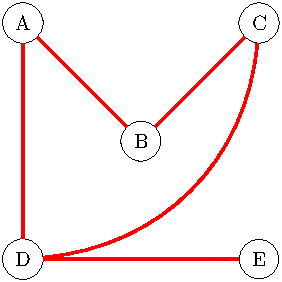
\includegraphics{graph1}
  \end{center}
  \vspace*{\fill}
  \begin{solution}
    Yes. Color the graph like this:
    \begin{center}
      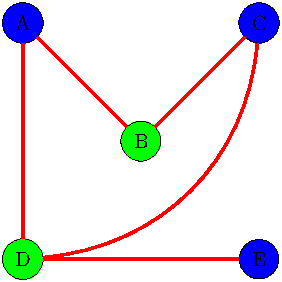
\includegraphics{graph1colored}
    \end{center}

    Or you can put the nodes into sets such as:
    \begin{center}
      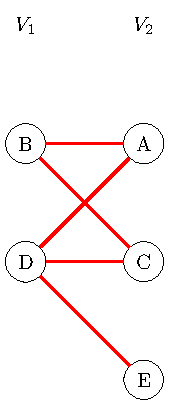
\includegraphics{graph1sets}
    \end{center}
  \end{solution}

  \question For the following graph find a path with no repeated edges from $d$ to $e$ containing all edges. (Or explain why it doesn't exist)
  \begin{center}
    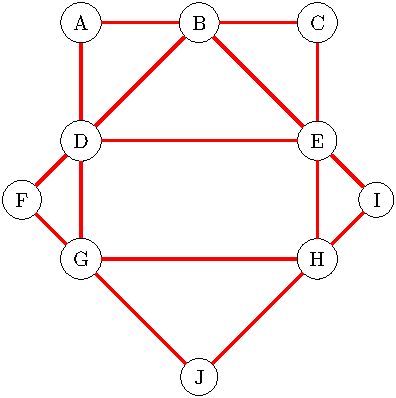
\includegraphics{graph2}
  \end{center}
  \vspace*{\fill}
  \begin{solution}
    The path is long and repeats nodes, (in fact going from $D$ to $E$ numerous times) but:
    \[
      D\to F \to G \to J \to H \to I \to E \to B \to D \to A \to B \to C \to E \to H \to G\to D\to E
    \]

    Or on a graph with edges numbered:
    \begin{center}
      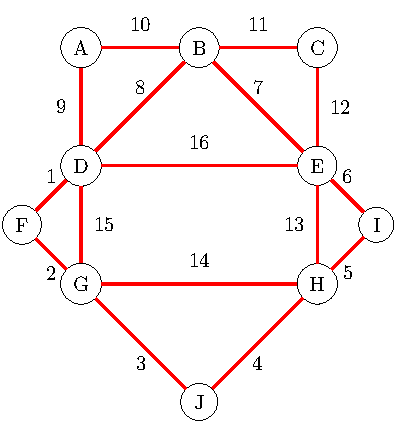
\includegraphics{graph2numbered}
    \end{center}
  \end{solution}
\end{questions}
\end{document}
